\documentclass[journal]{IEEEtran}

\usepackage[T1]{fontenc}
\usepackage[utf8]{inputenc}
\usepackage{xcolor,soul,framed}
\colorlet{shadecolor}{yellow}
\usepackage{graphicx}
\graphicspath{{figures/}}
\usepackage[cmex10]{amsmath}
\usepackage{array}
\usepackage{url}
\usepackage{cite}

\hyphenation{op-tical net-works semi-conduc-tor}

\begin{document}

\title{This is a first test with the demo repo}
\author{First Author$^{1,2}$,
        Second Author$^{2}$,
        Third Author$^{1}$,
        and Corresponding Author$^{1}$,~\IEEEmembership{Member,~IEEE}
\thanks{$^{1}$Instituto Politecnico Nacional, UPALM, Edif. Z-4 3er Piso,
  Ciudad de Mexico, 07738, Mexico}
\thanks{$^{2}$Departament d'Enginyeria Electronica, Universitat Autonoma
  de Barcelona, Bellaterra, 08193, Spain}
\thanks{Corresponding author e-mail: authorname@ipn.mx}}

\maketitle

\begin{abstract}
This manuscript demonstrates a collaborative workflow for writing IEEE
journal papers with local {\LaTeX}, Git, and visual revision tracking.
Replace this abstract with a concise summary of your contributions,
methods, and main results.
\end{abstract}

\begin{IEEEkeywords}
Collaborative writing, Git, IEEE, {\LaTeX}, version control
\end{IEEEkeywords}

\section{Introduction}

\IEEEPARstart{I}{n} the coming years, research teams will increasingly
rely on version control to manage manuscript revisions. This template
is a minimal IEEE journal starting point that compiles with
\texttt{latexmk} and works well with VS~Code and {\LaTeX} Workshop.

Sample citations appear as~\cite{example2020,example2022,lamport1994}.

\section{Proposed Approach}

The proposed approach combines local compilation, Git commits for every
meaningful edit, and \texttt{git-latexdiff} (or the LaTeX Diff editor
extension) to produce colored PDFs between any two revisions.

\begin{figure}[!t]
\centering
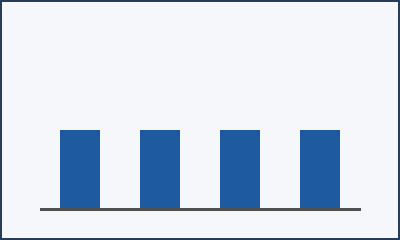
\includegraphics[width=0.85\columnwidth]{sample_plot.png}
\caption{Placeholder figure used to exercise image inclusion and
  whole-tree \texttt{git-latexdiff} runs.}
\label{fig:sample}
\end{figure}

Fig.~\ref{fig:sample} shows a sample plot stored under
\texttt{figures/}. Replace it with your own graphics and keep stable
filenames across revisions.

\section{Results}

A first pass over the sample data shows a clear upward trend in
Fig.~\ref{fig:sample}. Report effect sizes and confidence intervals
here when you replace this placeholder.

\section{Conclusion}

The sample workflow is enough for a small co-author team to compile
locally, share commits on GitHub, and produce a colored revision PDF.
Replace this paragraph with your own findings and future work.

\section*{Acknowledgment}

The authors would like to thank colleagues who tested this collaborative
{\LaTeX} workflow.

\bibliographystyle{IEEEtran}
\bibliography{refs}

\end{document}
